\section{Referenzarchitektur}\label{theorie:referenzmodellierung}
Nach \citeauthor{Bass.2010} ist eine Referenzarchitektur ein spezialisiertes Referenzmodell, wie in \autoref{abb:RelationshipsReferenceModel} welches in Softwarearchitekturen instanziiert werden kann. \footcite[Vgl.][S.~17~f.]{Bass.2010} 

\begin{figure}[H]
\centering
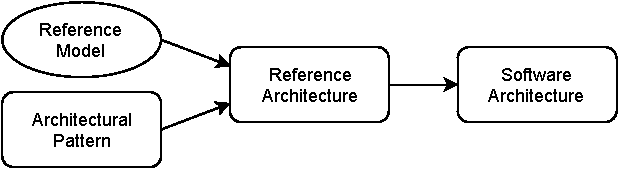
\includegraphics[width=0.66\textwidth]{graphics/Relationships-reference-models.pdf}
\caption[Beziehungen zwischen Referenzmodellen, Architekturpatterns, Referenzarchitekturen und Softwarearchitekturen]{Beziehungen zwischen Referenzmodellen, Architekturpatterns, Referenzarchitekturen und Softwarearchitekturen.\footnotemark}
\label{abb:RelationshipsReferenceModel}
\end{figure}
\footnotetext{Mit Änderungen entnommen aus: \cite[][18]{Bass.2010}}

In diesem Kapitel sollen deshalb die theoretische Definition des Referenzarchitekturbegriffs, genauso wie mögliche Vorgehensmodelle betrachtet werden.



\subsection{Referenzmodelle}

Gemäß des konstruktionsprozessorientierten Referenzmodellbegriffs von \citeauthor{vomBrocke.2003} ist ein Referenzmodell als solches zu erkennen, wenn der Gegenstand und/oder\footnote{Die Verwendung von \enquote{und/oder} wurde hier gewählt, da der Autor der Quelle das \enquote{oder} aus der boolschen Algebra gewählt hat um explizit beide Fälle einzuschliessen.} der Inhalt des Referenzmodells bei der Konstruktion des Gegenstandes und/oder des Inhaltes eines zu konstruierenden Anwendungsmodells wiederverwendet werden kann.\footcite[Vgl.][34]{vomBrocke.2003} Dabei hat ein Referenzmodell einen Empfehlungscharakter und stellt eine \enquote{best practice} dar.\footcite[Vgl.][31]{vomBrocke.2003} 

Ein Referenzmodell kann nach \citeauthor{vomBrocke.2003} nicht objektiv allgemeingültig sein und auch keinen objektiven Empfehlungscharakter haben, sondern muss subjektiv beurteilt werden.\footcite[Vgl. auch im Folgenden][31~f.]{vomBrocke.2003}  Dabei ist zumindest von den Interessensgruppen der Konstruierenden und der Nutzenden auszugehen, welche das Referenzmodell subjektiv unterschiedlich nach Allgemeingültigkeit und Empfehlungscharakter bewerten. Je nachdem welche Beurteilung höher gewichtet wird und früher einfließt, kann also entweder von der Situation ausgegangen werden, dass das Referenzmodell vom Konstruierenden zu einem solchen erklärt wird oder ein Modell, ob vom Konstruierenden beabsichtigt oder nicht, von den Nutzenden zu einem solchen erhoben wird.

\subsection{Grundsätze ordnungsgemäßer Referenzmodellierung}
\Todo{Grundsätze ordnungsgemäßer Modellierung/GoRM - siehe auch 148 vomBrocke.2003} \\
\textbf{=> Buch ist per Fernleihe bestellt, aber noch nicht da}


\subsection{Referenzarchitektur}
Der IEEE Standard 1471-2000 definiert Architektur im Kontext von softwareintensiven Systemen wie folgt:
\enquote{The fundamental organization of a system embodied in its components, their relationships
to each other, and to the environment, and the principles guiding its design and evolution.} \footcite[][3]{IEEEComputerSociety.2000}. Ein softwareintensives System wird dabei als jedes System, bei dem Software essentielle Einflüsse auf das Design, die Erstellung, das Deployment oder die Evolution des Systems hat.\footcite[Vgl.][1]{IEEEComputerSociety.2000}

Wird dieser Architekturbegriff auf bekannte Bereitstellungsmodi aus der Cloud, wie \ac{SaaS}, \ac{PaaS}, \ac{IaaS} oder \ac{FaaS} angewendet, wird klar, dass von einer Architektur im Sinne des IEEE Standards 1471-2000 ausgegangen werden kann, sobald Software involviert ist. Im Rahmen dieser Arbeit werden auch Dienste, die sich nach der NIST Cloud Definition unter \ac{SaaS} Dienste zählen lassen, behandelt. Als \ac{SaaS} Dienst gilt dabei jeder Dienst, bei dem Nutzende die unterliegende Infrastruktur nicht verwalten und die Applikation nur über limitierte Konfigurationen verwalten können. Sollte aber die Konfiguration mittels einer Programmiersprache bzw. Datenabfragesprache wie SQL erfolgen, ist die Bedingung erfüllt, dass Software wesentliche Einflüsse auf das System hat.


\citeauthor{Gallagher.2000} definiert eine Referenzarchitektur als eine generalisierte Architektur mehrerer Endsysteme, die eine oder mehrere Domänen teilen.\footcite[Vgl. auch im Folgenden][3]{Gallagher.2000} Die Referenzarchitektur definiert nach Sicht des Autors dabei die gemeinsame Infrastruktur der Endsysteme und die Schnitstellen der Komponenten, die in den Endsystemen enthalten sein sollen. Dabei ist eine Referenzarchitektur zu instanziieren, um eine spezifische Softwarearchitektur zu erstellen. Gallagher definiert die Aufgaben einer Referenzarchitektur wie folgt: Zum einen werden übergreifende Funktionen und Konfigurationen generalisiert und extrahiert und zum anderen wird eine kosteneffiziente und verlässliche Basis geschaffen, um Zielsysteme abzuleiten/zu instanziieren.\footcite[Vgl.][3]{Gallagher.2000}

\citeauthor{Trefke.2012} schränkt in seiner Definition die Instanziierung insoweit ein, dass individuelle Besonderheiten abstrahiert werden müssen, um eine Allgemeingültigkeit der Referenzarchitektur in einer speziellen Domäne zu erhalten.  \footcite[Vgl. auch im Folgenden][]{Trefke.2012} Zusätzlich fügt \citeauthor{Trefke.2012} der Referenzarchitektur als optionale Aufgaben die Definition von Leitlinien für die Verwendung, Evolution und Verantwortlichkeiten hinzu. Zurückgreifend auf \citeauthor{vomBrocke.2003} legt \citeauthor{Trefke.2012} fest, dass eine Referenzarchitektur als spezifischeres Referenzmodell seinen Empfehlungscharakter entweder durch Erfahrungen und hohe Nutzerakzeptanz oder durch Festsetzung durch Erschaffende erhält.

Nach \citeauthor{Angelov.2012} gibt es zwei Typen und damit verbundene Zielsetzungen der Referenzarchitektur: Die standardisierende Referenzarchitektur, welche darauf zielt eine Standardarchitektur für spezielle Anwendungsfälle zu schaffen und die unterstützende/erleichternde Referenzarchitektur, welche Personen in Architekturrollen unterstützen sollen, ähnliche Probleme leichter zu lösen.\footcite[Vgl. auch im Folgenden][S.~422~ff.]{Angelov.2012} Nach \citeauthor{Angelov.2012} sind standardisierende Referenzarchitekturen nicht zur Verwendung von innovativen, also kaum getesteten oder noch nicht von Experten akzeptierten Elementen geeignet. Die unterstützenden/erleichternden Referenzarchitekturen hingegen können solche innovativen Elemente durchaus verwenden und auch eine Technologievorauswahl treffen.

% Um einen möglichst hohen Nutzen stiften zu können, müssen die organisatorischen Rahmenbedingungen, in welchen ein Referenzmodell eingesetzt werden soll analysiert werden.\footcite[Vgl.][]{vomBrocke.2004}

%\Todo{What are inputs of a Reference Architecture? - Muller.2020}
\citeauthor{Muller.2020} empfiehlt eine Referenzarchitektur zur Generalisierung von vorhandenen Architekturen zu verwenden, schlägt aber für neue Technologien und Applikationen, die bislang in der Form kaum verwendet wurden ein inkrementelles Vorgehen vor.\footcite[Vgl. auch im Folgenden][7]{Muller.2020} Das inkrementelle Vorgehen von Muller beinhaltet dabei die Erstellung von Prototypen und inkrementelle Einholung von Feedback der Zielstakeholder.


\subsection{Qualitätskriterien von Referenzarchitekturen}\label{chap:qualitycriteria}
\citeauthor{Muller.2020} schlägt sieben Qualitätskriterien vor, welche von einer guten Referenzarchitektur erfüllt werden sollten:\footcite[Vgl. auch im Folgenden][8]{Muller.2020}
\begin{enumerate}
\item Verständlichkeit für eine breite, heterogene Gruppe an Stakeholdern (Kunden, Projektmanager, Entwickler, etc.)
\item Zugänglichkeit und Zugriff durch die Mehrheit der Organisation
\item Adressierung der Hauptprobleme der spezifischen Problemdomäne
\item Zufriedenstellende Qualität
\item akzeptabel
\item \enquote{up-to-date} und wartbar
\item wertschöpfend für den Betrieb
\end{enumerate}

\ac{AWS} definiert im Rahmen des sogenannten Well Architected Frameworks für verschiedene \enquote{Lenses}, also Spezialisierungen, Themenfelder, die bei exzellenten Architekturen zu beachten sind. Für Datenanalysen gibt es die Analytics Lens, welche entsprechend für Referenzarchitekturen genauso Anwendung finden sollte. Kriterien sind dabei die Folgenden:\footcite[Vgl.][6]{Ravirala.2020}:
\begin{itemize}
\item Automate data ingestion
\item Design ingestion for failures and duplicates => Siehe Robustness and fault tolerance
\item Preserve original source data
\item Describe data with metadata
\item Establish data lineage
\item Use the right ETL tool for the job
\item Orchestrate ETL workflows
\item Tier storage appropriately
\item Secure, protect, and manage your entire analytics pipeline
\item Design for scalable and reliable analytics pipelines => Scalability, robustness and fault tolerance
\end{itemize}


\subsection{Vorgehensmodell}

\citeauthor{Schutte.1998} unterteilt Referenzmodellierung generell in vier Phasen.\footcite[Vgl. auch im Folgenden][184\psq]{Schutte.1998} Die erste Phase, die Problemdefinition ist mit der Darstellung des behandelten Problems in der Einleitung dieser Arbeit bereits vorgenommen worden. Laut \citeauthor{Schutte.1998} kann der Wirklichkeitszugang des erstellten Modells nur über Bilder erfolgen, welche entsprechend zu modellieren sind.\footcite[Vgl. auch im Folgenden][185\psq]{Schutte.1998} Da momentan keine Erfahrungen in den zu verwendenden Technologien für die Referenzmodellierung vorliegt, handelt es sich um eine Top-down Referenzmodellierung/Referenzarchitektur.

\begin{figure}[H]
\centering
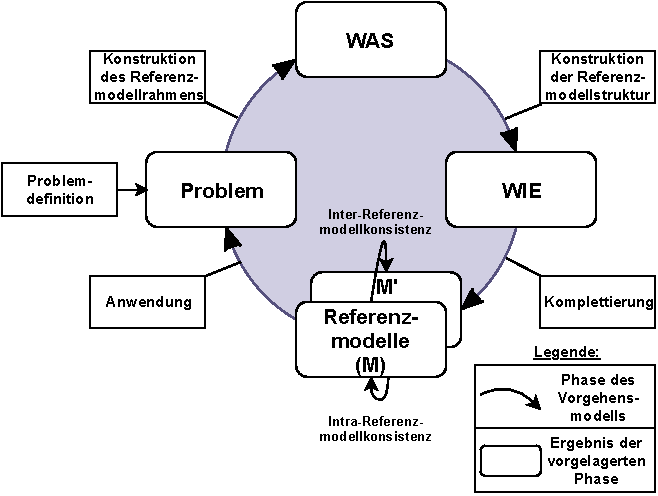
\includegraphics[width=0.75\textwidth]{graphics/Vorgehen-Referenzmodellierung.pdf}
\caption[Vorgehensmodell Referenzmodellierung nach Schütte]{Vorgehensmodell Referenzmodellierung nach Schütte.\footnotemark}
\label{abb:VorgehensmodellReferenzmodellierung}
\end{figure}
\footnotetext{Mit Änderungen entnommen aus: \cite[][185]{Schutte.1998}}




Nach \citeauthor{Muller.2020} hat eine Referenzarchitektur mehrere Dekompositionen, in beispielsweise eine funktionale, eine konstruktionsorientierte oder eine infrastrukturorientierte Komposition. Diese Dekompositionsschichten lassen sich ebenfalls in bekannten Architekturfframeworks wie arc42 finden, weshalb diese mit Anpassungen zur Visualisierung dienen sollen. Dies deckt sich auch mit der Auffasung von \citeauthor{Schutte.1998} zur Referenzmodellierung.

Zur Darstellung der verwendeten Produkte und Dienstleistungen von \ac{AWS} in den Referenzarchitekturen und dem Datenfluss soll die erste Stufe der Bausteinsicht des Architekturstandards arc42 verwendet werden. Das Konzept jener Bausteinsicht, also wie sie zu gestalten ist, findet sich in \autoref{abb:BausteinsichtStufe1}. In der finalen Umsetzung werden die offiziellen \ac{AWS} Icons die entsprechenden Services darstellen, die verwendet werden. Weitere Dekompositionsebenen, Beispiele und Kentnissammlungen die zu einer Referenzarchitektur gehören können unformalisierter beigefügt werden.

\begin{figure}[H]
\centering
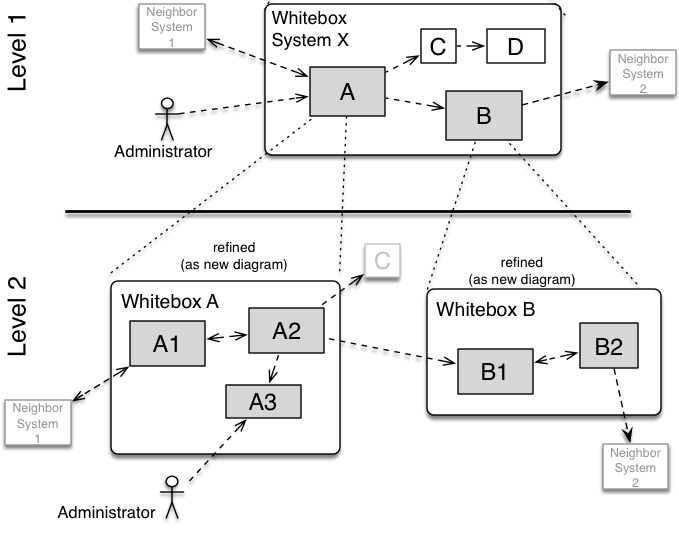
\includegraphics[width=\textwidth]{graphics/Bausteinsicht.png}
\caption[Stufe 1 der Bausteinsicht in arc42]{Stufe 1 der Bausteinsicht in arc42.\footnotemark}
\label{abb:BausteinsichtStufe1}
\end{figure}
\footnotetext{Mit Änderungen entnommen aus: \cite{Starke.o.J.}}



Wie von \citeauthor{Muller.2020} vorgeschlagen und im vorherigen Unterkapitel erläutert, ist ein inkrementeller Ansatz unter Verwendung von Prototypen und kontinuierlichem Feedback der Zielstakeholder unerlässlich.\footcite[Vgl.][7]{Muller.2020} 

Sehr wichtig für eine Referenzarchitektur ist auch die Dokumentation, wie die Wiederverwendung zu handhaben ist. Ein möglicher Ansatz wäre dabei die gezielte Integration und Dokumentation von Variationspunkten, wie von \citeauthor{Webber.2001} vorgeschlagen.\footcite[Vgl.][24\psqq]{Webber.2001} Mittels der Variationspunkte kann eine statische Referenzarchitektur konstruiert werden, welche an spezifisch definierten Punkten angepasst werden muss, um einzigartige Architekturen zu erzeugen.\footcite[Vgl.][24]{Webber.2001} Dabei gibt es vier verschiedene Ansichten, aus denen Variationspunkte definiert werden können:\footcite[Vgl.][25\psq]{Webber.2001}
\begin{enumerate}
\item \label{view:first} Requirement-Variation-Point View
\item \label{view:second} Component-Variation-Point View
\item \label{view:third} Static-Variation-Point View
\item \label{view:fourth} Dynamic-Variation-Point View
\end{enumerate}
Dabei sind für diese Arbeit, in der keine implementierungsnahe (im Sinne von Programmierung) Softwarearchitektur entworfen wird, hauptsächlich die anforderungsbasierte und die komponentenbasierte Variationspunktsicht aus \autoref{view:first} und \autoref{view:second} wichtig. Die statische und dynamische Variationspunktsicht aus \autoref{view:third} und \autoref{view:fourth} agieren stärker auf Implementierungsebene, in dem beispielsweise mittels objektorientierter Programmierung Klassen bereitgestellt werden, von welchen geerbt werden kann und deren Verhaltensweisen durch z.B. Callbacks oder Parameterisierung des Aufrufes verändert werden kann.\footcite[Vgl.][25\psq]{Webber.2001} 

\renewcommand\#{\protect\scalebox{0.8}{\protect\raisebox{0.4ex}{\char"0023}}}

Variationspunkte können, wie in \autoref{abb:Variationspunkte} dargestellt innerhalb der verschiedenen, dargestellten Schichten wie folgt dargestellt werden:
\begin{figure}[H]
\centering

\includegraphics[height=1.33cm]{graphics/Variationpoints.pdf}
\caption{Darstellung Variationspunkte}
\label{abb:Variationspunkte}
\end{figure}
In den Architekturebenen werden entsprechend die Variationspunkte mit durchgängigen Nummern versehen, welche entsprechend vor dem \# stehen.





% Überleitung => generelle Referenzmodelle 
% => Empfehlungscharakter 
% => Anwendung Architektur 
% => Unterlegung Arc42 als Modellierungssprache

